\chapter{Diseño, Seguimiento y Control}
\label{chap:diseño} 

ARxCODE resulta una aplicaci\'on de escritorio, de estructura modular, reusable y modificable. Pensada con una filosof\'ia de expansi\'on y perfeccionamiento, su arquitectura permite la adici\'on de funcionalidades sin mayores inconvenientes.\\

\section{Arquitectura}

\subsection*{Componentes}\label{subsec:componentes}
En un planteo conceptual, con alto grado de abstracci\'on, los distintos paquetes de ARxCODE pueden agruparse en cinco componentes (Fig.  \ref{fig:componentes}): PROCESAMIENTO, ADMINISTRACI\'ON DE DATOS, INTERFAZ GR\'AFICA Y VISUALIZACI\'ON, Sistemas de Referencia y VALIDACIONES.

\begin{itemize}
 \item PROCESAMIENTO: Involucra los cuatro paquetes que, no s\'olo operan con los datos ingresados, sino que tambi\'en los manipulan y procesan para generar nuevos productos. Estos m\'odulos son, de alguna manera, los distintos n\'ucleos del c\'odigo.\\

 \begin{itemize}
 \itemsep0em
  \item {\it{AjustarTle}}
  \item {\it{Comparar}}
  \item {\it{Estadistica}}
  \item {\it{Encuentro}}
 \end{itemize}

 \item ADMINISTRACI\'ON DE DATOS: Son aquellos paquetes que se encargan de la obtenci\'on, el desglose y el preprocesamiento de los datos que ser\'an utilizados por el resto de los m\'odulos.

 \begin{itemize}
 \itemsep0em
  \item {\it{TleAdmin}}
  \item {\it{CodsAdmin}}
  \item {\it{CDM}}
 \end{itemize}

 \item INTERFAZ Y VISUALIZACI\'ON: Agrupa el paquete que genera la interfaz gr\'afica y el paquete que contiene todos los m\'odulos que generan representaciones visuales, como los gr\'aficos o las proyecciones de las trayectorias sobre el mapa.\\
 \begin{itemize}
 \itemsep0em
 \item {\it{Aplicacion}}
 \item {\it{visual}}
 \end{itemize}
 \item Sistemas de Referencia: {\it{SistReferencia}}, es el paquete que contiene todo lo referente a las transformaciones entre los distintos sistemas de referencia, ya sean espaciales o de tiempo.
 \item VALIDACIONES: Agrupa todos los m\'odulos desarrollados para validar los resultados.
\end{itemize}


\begin{figure}[h!]
  \centering
  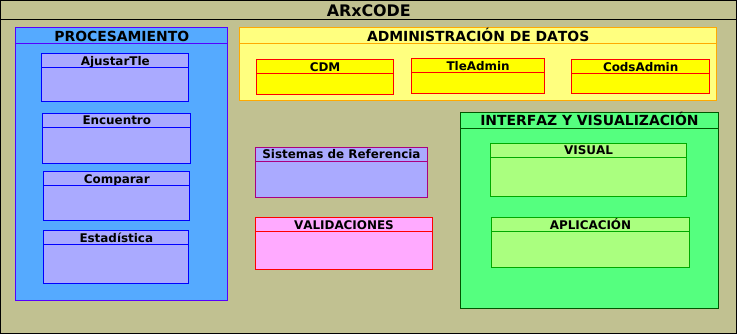
\includegraphics[width=0.7\textwidth]{imagenes/componentesAR}  
  \caption{Componentes de ARxCODE}
  \label{fig:componentes}
\end{figure}

\subsubsection*{ADMINISTRACI\'ON DE DATOS: TleAdmin}
Este paquete contiene las dos clases que gestionan la descarga de los TLEs de la p\'agina Space-Track: {\bf{Tle}} y {\bf{setTLE}} (Fig. \ref{fig:Tleadmin}). La primera provee un \'unico TLE y todo lo referente a \'el; se instancia a partir del identificador de NORAD del objeto y una \'epoca, o a partir del nombre de un archivo que contiene un \'unico TLE. Entre sus m\'etodos, es fundamental {\bf{propagaTLE()}}, que propaga la posici\'on del objeto al momento que sea necesario.\\

La clase {\bf{setTLE}}, es necesaria particularmente para la implementaci\'on del m\'etodo de Osweiler que requiere un conjunto de TLEs de 15 d\'ias para la generaci\'on de la matriz de covarianza de la posici\'on del objeto. Esta clase se instancia, indicando el identificador de NORAD del objeto, la fecha de inicio y fin, del set que se requiere. Una vez descargados, genera un \'unico archivo con todos los TLEs del intervalo y los guarda en la carpeta {\it{crudosTLE}}.\\

El m\'etodo {\bf{divide\_setTLE()}} de la clase {\bf{setTLE}}, particiona el texto con el conjunto de TLEs y genera un archivo por cada TLE y lo almacena en la carpeta {\it{tle}} del paquete.
Esta \'ultima carpeta, se actualiza con cada corrida del software, de modo que siempre contiene s\'olo el conjunto de archivos de TLEs que van a ser procesados.\\

\begin{figure}[!h]
\centering
  \subfigure[Clase TLE (TleAdmin/TLE/Tle)]{
    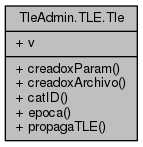
\includegraphics[width=0.3\textwidth]{imagenes/tleClass}
  }
  \hspace{1.5cm}
  \subfigure[Clase setTLE (TleAdmin/TLE/setTLE)]{
    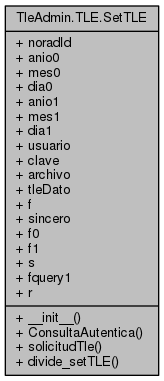
\includegraphics[width=0.3\columnwidth, keepaspectratio]{imagenes/setTLEclass}
  }
  \caption[Clases Tle y setTLE]{Clases Tle y setTLE del paquete TleAdmin}
  \label{fig:Tleadmin}
\end{figure}

\subsubsection*{ADMINISTRACI\'ON DE DATOS: CDM}
El paquete CDM contiene una carpeta con archivos en formato del CDM, en xml y la clase {\bf{CDM}} que tiene la capacidad de desglozarlos y extraer los datos del mensajes que ser\'an plasmados en la pantalla de la interfaz gr\'afica, para la visualizaci\'on del operador.\\

\subsubsection*{ADMINISTRACI\'ON DE DATOS: CodsAdmin}
Este paquete administra los productos orbitales generados por el departamento de Din\'amica Orbital \ac{CODS}.
Cuenta con varias carpetas que almacenan los productos previamente descargados y contiene a la clase {\bf{EphemCODS}}, que tiene la capacidad de extraer las efem\'erides de los archivos y de identificar el periodo de datos que abarca el archivo a partir del nombre.\\

\begin{figure}[!h]
\centering
  \subfigure[Clase CDM (CDM/CDM).]{
    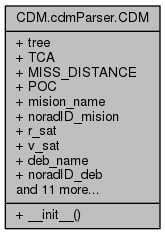
\includegraphics[width=.3\textwidth]{imagenes/cdmClass}
    \label{fig:clasetle}
  }
  \hspace{1.5cm}
  \subfigure[Clase EphemCODS (CodsAdmin/EphemCODS)]{
    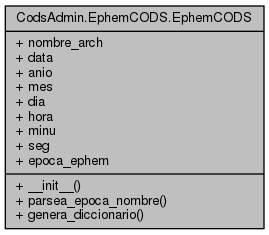
\includegraphics[width=0.4\columnwidth, keepaspectratio]{imagenes/ephemcodsClass}
    \label{fig:clasesettle}
  }
  \caption[Clases CDM y EphemCODS]{Clases CDM y EphemCODS para el pareseo de los mensajes de alerta CDM y los productos orbitales de \ac{CODS}}
\end{figure}

\subsubsection*{PROCESAMIENTO: AjustarTle}
Este paquete incluye el m\'odulo con el mismo nombre {\it{AjustarTle}}, que cuenta con varias funciones que reagrupan la informaci\'on del conjunto de TLEs a fin de poder hacer ordenamientos y comparaciones, entre los TLE de distintas fechas que son propagados a una misma \'epoca (pr\'actica necesaria para la implementaci\'on del m\'etodo de Osweiler para la construcci\'on de las matrices de covarianza).\\

\subsubsection*{PROCESAMIENTO: Comparar}
En el paquete {\it{Comparar}} se nuclean todos los m\'odulos y funciones que permiten la selecci\'on y la extracci\'on de los datos de los productos de Din\'amica Orbital (CODS), y sus respectivas comparaciones con los resultados que provienen de la propagaci\'on de los TLEs. Este tipo de comparaciones son necesarias en la estimaci\'on de errores que se comenten al utilizar propagaciones de los TLE con SGP4. 

\subsubsection*{PROCESAMIENTO: Estad\'istica}
Dentro de este paquete se encuentran los desarrollos referidos a los c\'alculos estad\'isticos, m\'as precisamente los m\'odulos que calculan las matrices de covarianza. En este paquete se encuentra el m\'odulo que implementa el m\'etodo de Osweiler, \citep{osweiler} {\bf{matrizOsweiler()}}.

\subsubsection*{PROCESAMIENTO: Encuentro}
Este es el paquete n\'ucleo del software. En \'el se encuentra la clase {\bf{Encuentro}}  (Fig. \ref{fig:claseencuentro}), que instancia la generaci\'on del encuentro, incorporando ambos objetos mediante sus identificadores de NORAD y el TCA, generando las propagaciones necesarias, y las matrices de error, para calcular la m\'inima distancia y la probabilidad de colisi\'on. A tal fin, cuenta con los m\'etodos (Fig. \ref{fig:claseencuentro}): {\bf{calculaMacombinada()}}, {\bf{proyecta\_alplano\_encuentro()}}, {\bf{calculaPoC\_circ()}} y  {\bf{calculaPoC\_gral()}}\\

\begin{figure}[h!]
  \centering
  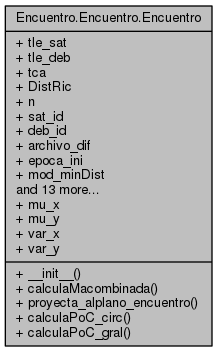
\includegraphics[width=.3\textwidth]{imagenes/encuentroClass} 
  \caption[Clase Encuentro]{Clase Encuentro para el c\'alculo de los par\'ametros del acercamiento}
  \label{fig:claseencuentro}
\end{figure}


\subsubsection*{INTERFAZ GR\'AFICA Y VISUALIZACI\'ON: Aplicaci\'on}
Este paquete contiene, principalmente el m\'odulo con el formulario de interfaz de ARxCODE {\bf{frm\_main}}. Dentro del mismo se ubican las clases que heredan de la estructura de QT, para el desarrollo de la aplicaci\'on, y son estas clases las que invocan los distintos m\'odulos del resto del c\'odigo para el desarrollo de los procesos.\\

\subsubsection*{INTERFAZ GR\'AFICA Y VISUALIZACI\'ON: visual}
{\bf{Visual}} es el paquete que agrupa todos los m\'odulos de generaci\'on de gr\'aficos y ploteos. Los gr\'aficos se utilizaron principalmente para el estudio de la tendencia de errores de los TLE y otros an\'alisis y validaciones.
Dentro de este paquete se encuentra el m\'odulo que genera las trayectorias de las \'orbitas, proyectadas sobre el mapa en el momento del encuentro.\\

\subsubsection*{Sistemas de Referencia}
Este paquete contiene m\'odulos para realizar transformaciones entre los distintos sistemas de referencia. Entre ellos, los dos m\'as utilizados son:
{\it{teme2tod}} y {\it{ricSis}}, ya descriptos en la Sec. \ref{subsec:sistRef}.

\subsubsection*{Validaciones}
Re\'une todos los m\'odulos que se desarrollaron para la verificaci\'on y validaci\'on de los resultados que se describen a continuaci\'on (Sec. \ref{lab:vandv}), y cuyos valores se analizan y publican en la secci\'on de Resultados y Validaciones (Sec. \ref{chap:resultados}).

\section{Interfaces}
Por cuestiones de tiempo y de accesibilidad, para el desarrollo de este trabajo, los datos que provee el departamento de Din\'amica Orbital fueron descargados y se extraen de un directorio, al igual que los mensajes de alerta CDM, que fueron descargados de p\'aginas de internet , ya que no nos han facilitado ninguno vinculado a la misi\'on operativa con la que trabajamos, por motivos de confidencialidad.\\

Se realiz\'o la automatizaci\'on de la descarga de TLEs de la p\'agina Space-Track y se habilit\'o en la interfaz la pantalla que permite la carga manual de los datos del encuentro. Como resultado, las interfaces implementadas, son (Fig. \ref{fig:interfacesImpl}):
 
\begin{itemize}
\itemsep0em
 \item Conexi\'on a Space-Track para la solicitud de TLEs.
 \item Administraci\'on de las efem\'erides orbitales de los directorios de CodsAdmin.
 \item Administraci\'on de los CDM del directorio CDM, a trav\'es de la intervenci\'on del operador.
 \item Carga Manual de datos de un encuentro realizada por el operador.
\end{itemize}

\begin{figure}[!h]
\centering
  \fbox{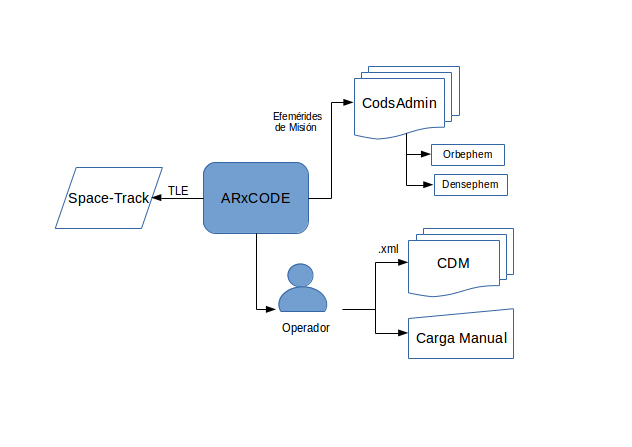
\includegraphics[width=0.6\textwidth]{imagenes/interfazImplementada}}
  \caption[Diagrama de Interfaces Implementadas en ARxCODE]{Diagrama de Interfaces Implementadas en ARxCODE}
  \label{fig:interfacesImpl}
\end{figure}

% \subsection*{Pantallas del ARxCODE}
% 
% Se muestran a continuaci\'on las pantallas del sistema, en secuencia de acuerdo a las posibles operaciones.
% 
% \begin{figure}[!h]
%   \centering
%   \fbox{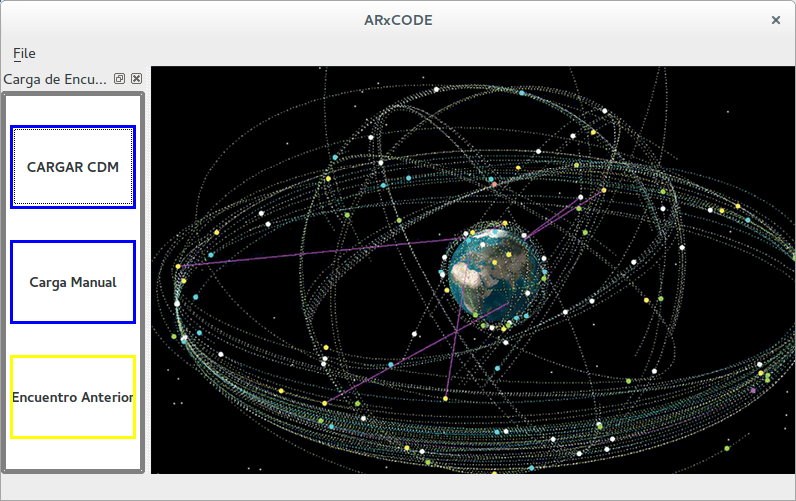
\includegraphics[width=0.8\textwidth]{imagenes/pantalla0}}
%   \caption{Impresi\'on de la pantalla de inicio del ARxCODE}
%   \label{fig:pantInicio}
% \end{figure}
% 
% \begin{figure}[h!]
%   \centering
%   \fbox{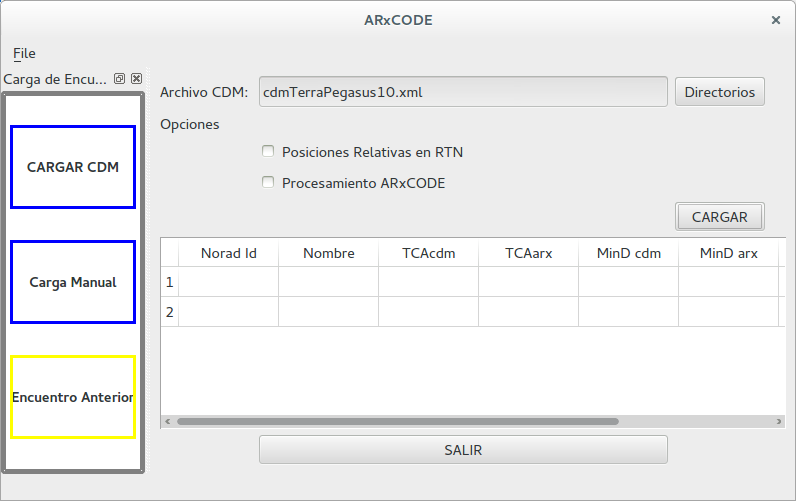
\includegraphics[width=0.8\textwidth]{imagenes/pantalla1}}
%   \caption{Impresi\'on de la pantalla de Procesamiento de CDM del ARxCODE.}
%   \label{fig:ingresadatosPant}
% \end{figure}
% 
% \begin{figure}[h!]
%   \centering
%   \fbox{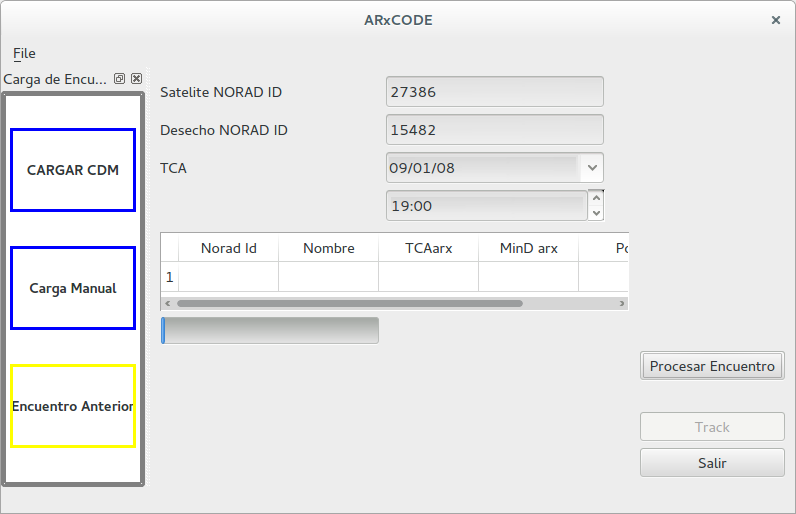
\includegraphics[width=0.8\textwidth]{imagenes/pantalla2}}
%   \caption{Impresi\'on de la pantalla del ingreso manual de datos del ARxCODE}
%   \label{fig:ingresadatosPant1}
% \end{figure}
% 
% \begin{figure}[h!]
%   \centering
%   \fbox{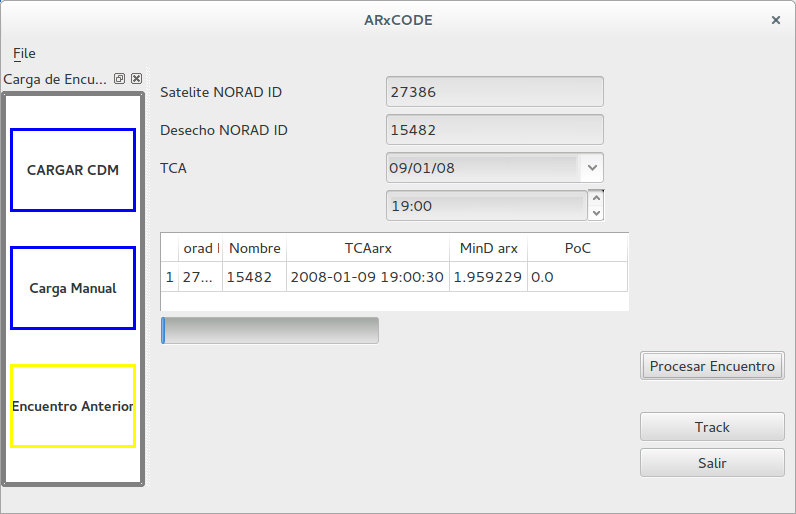
\includegraphics[width=0.8\textwidth]{imagenes/pantalla3}}
%   \caption{Vista con la carga del procesamiento manual.}
%   \label{fig:pantproc}
% \end{figure}
% 
% \begin{figure}[h!]
%   \centering
%   \fbox{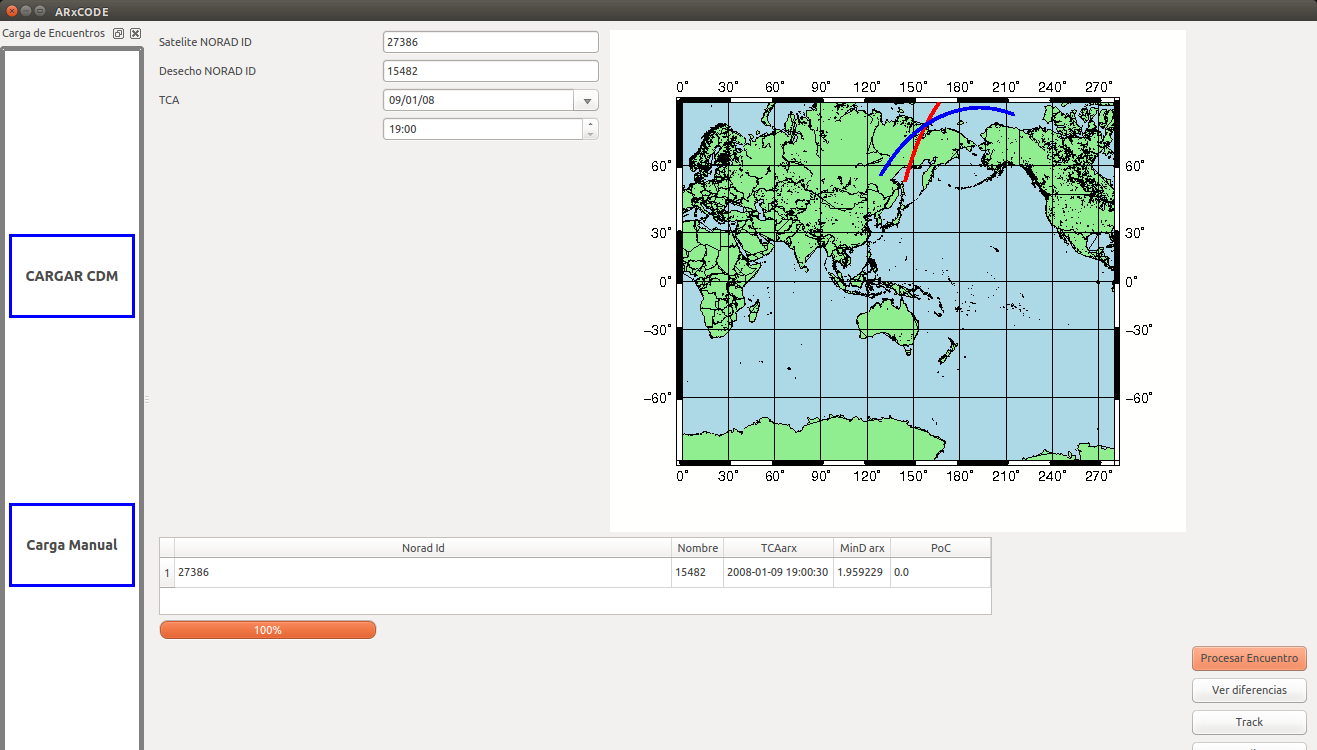
\includegraphics[width=0.8\textwidth]{imagenes/pantalla4}}
%   \caption{Vista con los resultados publicados y la incorporaci\'on de las trayectorias.}
%   \label{fig:pantfinal}
% \end{figure}

\section{Seguimiento y Control}

\subsection{Verificaci\'on y Validaci\'on}\label{sec:vandv}

\subsubsection*{Verificaci\'on}
Se realizaron distintas pruebas de unidad y de integraci\'on.  
Los distintos casos de prueba se diseñaban a partir de datos de prueba de la bibliograf\'ia recabada para cada una de las metodolog\'ias o sobre situaciones reales. Los resultados de la ejecución de las pruebas se comparaban luego con los valores de los casos publicados o la situaciones reales. Un breve esquema de este procedimiento puede verse en la Figura \ref{fig:metodoprueba}. 

\begin{figure}[h!]
  \centering
  \fbox{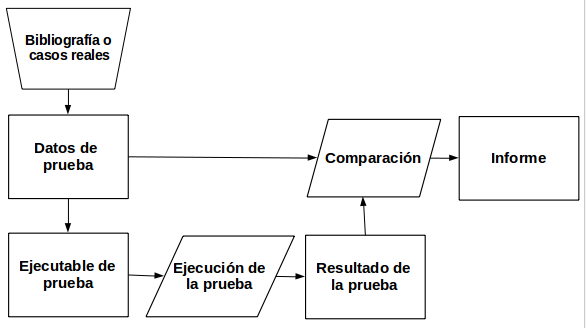
\includegraphics[width=0.7\textwidth]{imagenes/metodoprueba}}
  \caption{Esquema de la metodología para realizar las pruebas de unidad sobre los módulos.}
  \label{fig:metodoprueba}
\end{figure}

A medida que se desarrollaba un nuevo m\'odulo, se realizaban los casos de prueba para ese m\'odulo y una prueba de integraci\'on, que incorporaba todos los m\'odulos hasta el momento verificados.

\paragraph*{TleAdmin y CDM}
Dado que tanto los TLE como los CDM son los elementos fundamentales que dan inicio al an\'alisis de la probabilidad de colisi\'on, es fundamental tener un control sobre la correcta adquisici\'on de estos inputs. Sobre ellos se diseñaron pruebas funcionales. Se prueba siempre que los TLE de ambos objetos hayan sido adquiridos; si esto no fuera as\'i ya sea por complicaciones en la conexi\'on a internet, o porque los TLE para las fechas solicitadas no est\'an disponibles, el software interrumpe el proceso e indica a cu\'al de las situaciones se debe el problema. Mientras que para el caso de los CDM, el programa se interrumpe si el archivo ingresado no respeta el formato .xml capaz de procesar y anuncia un mensaje de alerta cuando el CDM a sido procesado pero no todos los campos de inter\'es se encuentran en \'el. 

\paragraph*{Comparar y SistReferencia}
Las pruebas realizadas para garantizar los correctos procedimientos respecto de la propagaci\'on y las transformaciones de los sistemas de referencia fueron fundamentales, pero s\'olo se realizaron en las primeras etapas del desarrollo, ya que no dependen de cada ejecuci\'on en particular, sino de la correcta implementaci\'on de los algoritmos.  

\paragraph*{Estad\'istica}
Para verificar la correcta implementaci\'on del m\'etodo de Osweiler para la generaci\'on de las matrices de covarianza, se gener\'o un caso de prueba que permite comparar los resultados con los que se publican en el trabajo del autor. Dada la dependencia de este m\'odulo con el m\'odulo de administraci\'on de los TLE, es importante que esta prueba es naturalmente de integraci\'on y es muy importante que se realice frecuentemente.

\paragraph*{Comparar y CodsAdmin}
El procedimiento que se realiza para la generaci\'on de la matriz de propagaci\'on de errores involucra la utilizaci\'on de los datos de misi\'on (o Datos de CODS). Esta tarea fue realmente compleja y se realizaron varias ejecuciones de la prueba sobre la manipulaci\'on de estos datos, ya que los mismos muchas veces no respetaban un formato estandarizado por ejemplo sobre las fechas o conten\'ian intervalos sin datos significativos, etc. Estas verificaciones se realizaron una sola vez hasta lograr que los datos resultaran ordenados dentro del per\'iodo de an\'alisis que se utiliz\'o para generar la matriz de propagaci\'on de errores. Por cuestiones de tiempo no se implement\'o una verificaci\'on automatizada sobre estos inputs, lo que debe ser tenido en cuenta si se desean generar matrices de propagaci\'on de errores actualizadas o en forma din\'amica.  

\paragraph*{Encuentro}
Las pruebas realizada en el m\'odulo para la estimaci\'on de las probabilidades de colisi\'on tienen tambi\'en una fuerte dependencia del m\'odulo que gestiona los TLE, mientras que pueden configurarse o no para que la matriz de covarianza que utilizan sea generada por el m\'odulo de Osweiler o no. Salvo para el caso del m\'etodo de Lei-Chen, ya que en su trabajo existe un ejemplo que indica todos los par\'ametros que se utilizan en la ecuaci\'on final, y entonces se puede hacer una prueba s\'olo para esa unidad.

\paragraph{Aplicaci\'on}
En lo que respecta a la aplicaci\'on que nuclea y despliega la interfaz gr\'afica, se realizaron inspecciones para depurar la correcta inicializaci\'on de variables y el flujo de las distintas vistas. 


\begin{figure}[!h]
\begin{minipage}[t]{0.48\textwidth}
 \centering
 \fbox{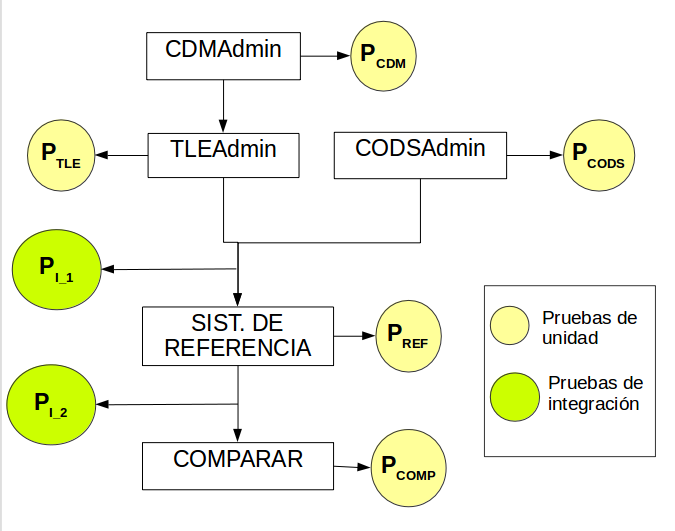
\includegraphics[width=0.9\textwidth]{imagenes/pruebasCods}}
 \caption[Casos de Prueba I]{Casos de prueba para los módulos que interactúan con los datos de Misión.}
 \label{fig:pruebaCods}
\end{minipage}
\begin{minipage}[t]{0.48\textwidth}
 \centering
 \fbox{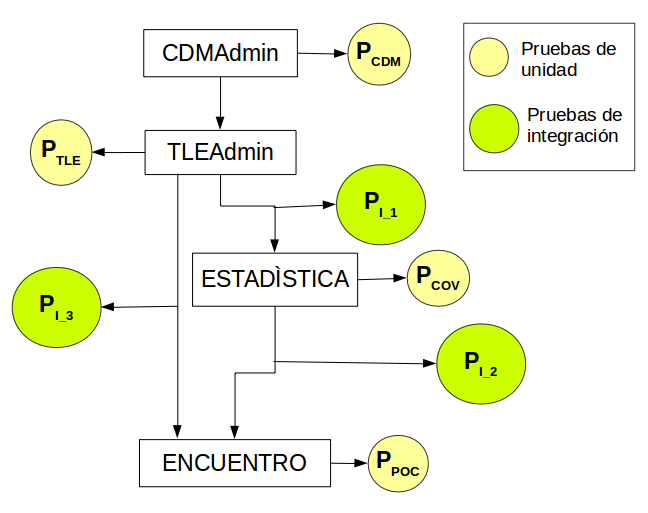
\includegraphics[width=0.9\textwidth]{imagenes/pruebasEncuentro}}
 \caption[Casos de Prueba II]{Casos de prueba del bloque completo, desde los inputs hasta el cálculo de la PoC.}
 \label{fig:pruebaEncuentro}
\end{minipage}
\end{figure}

\subsubsection*{Validaci\'on}

Al tratarse de un sistema que implementa distintas metodolog\'ias para el c\'alculo de par\'ametros, el control m\'as exhaustivo se bas\'o en analizar que los resultados de los algoritmos implementados fueran coherentes y coincidieran con los que exist\'ian en publicaciones bibliogr\'aficas o situaciones reales que se pod\'ian reproducir. \\

En conclusi\'on se han realizado distintas pruebas e inspecciones, pero no pruebas exhaustivas.
Un desarrollo detallado de los resultados de las pruebas y validaciones se describe en la Sec. \ref{chap:resultados}\\

\subsection{Gesti\'on de la Configuraci\'on}

Al ser ARxCODE un prototipo sencillo desarrollado por una sola persona, no fue necesario implementar una compleja gesti\'on de configuraci\'on. Se utiliz\'o el repositorio Git (Ver Sec. \ref{sec:entorno}) para el control de versiones, al que d\'ia a d\'ia se incorporaba el proyecto. Se paut\'o realizar un release una vez por mes, ya que era la frecuencia con la que se planific\'o que existieran nuevos m\'odulos y pruebas de unidad y/o de integraci\'on. 


\subsection{Aseguramiento de la Calidad}

Se han definido tres instancias fundamentales para la evaluaci\'on y el control de la calidad del software durante el desarrollo.

Sin duda el primer punto tiene que ver con el correcto acceso a los TLE que son los inputs b\'asicos para iniciar el procesamiento. Del mismo modo, la ingesta de un CDM defectuoso puede producir distintos fallos ya que al menos los m\'inimos datos de iniciaci\'on deben ser ingresados correctamente. Finalmente, todo el ciclo de los distintos procesos, a saber: solicitud de los TLE correspondientes, generaci\'on de matrices, c\'omputo de la m\'inima distancia y de la PoC, as\'i como todos los procesos de transformaciones de coordenadas deben realizarse en forma fluida.

A fin de garantizar un control sobre la calidad m\'inima en los puntos mencionados, una prueba general que contempla las tres pruebas integrales sobre el circuito completo se realiz\'o antes de cada release mensual. Con la misma frecuencia, a continuaci\'on se realizaron, pruebas sin acceso a internet y por ende sin acceso a la p\'agina proveedora de los TLE y sobre CDM defectuosos para verificar que el software interrump\'ia su proceder e informaba con un mensaje espec\'ifico a qu\'e se deb\'ia la interrupci\'on.

No obstante, a medida que se realizaban m\'as y m\'as pruebas, sumando nuevos datos de validaci\'on, otros puntos importantes fueron descubri\'endose. De modo que se incorporaron pruebas que permiten medir la diferencia de \'epocas entre el TLE y el tiempo de mayor acercamiento, a fin de garantizar que se informe al operador si las propagaciones orbitales superen los 7 d\'ias para el caso de las m\'inimas distancias, o los 15 d\'ias para la generaci\'on de matrices. 

En la misma direcci\'on fue importante incorporar un mensaje de alerta, cuando las matrices de covarianza generadas superan ciertos valores establecidos, ya que el proceso resulta finalizado exitosamente pero los datos no son confiables (Ver Tabla \ref{tab:pruebasQA}).

\begin{table}[!h]
\caption[Pruebas de Aseguramiento de la Calidad]{Pruebas de Aseguramiento de la Calidad que se realizaron antes de cada release, aproximadamente una vez al mes.}
\resizebox{17.5cm}{!}{
\begin{tabular}{cl}
\hline 
\rowcolor{lightgray}
\bf{Prueba}  &    \bf{Resultado esperado} \\
\hline
Prueba general & MSJ: {\it{El proceso ha finalizado correctamente}}\\
\hline
\makecell{Prueba sin internet \\ o sin devoluci\'on de TLE del sitio web} & INTERRUPI\'ON:  {\it{El TLE no se ha generado correctamente}}\\
\hline
Prueba con CDM defectuoso & INTERRUPI\'ON:  {\it{El CDM ingresado es incorrecto o est\'a incompleto}}\\
\hline
Prueba con TLE muy antiguos & MSJ de Alerta: {\it{El TLE utilizado en el problema no es de una \'epoca confiable}}\\
\hline 
\makecell{Prueba con matrices de covarianza\\ con errores groseros} & MSJ de Alerta: {\it{El TLE utilizado en el problema no es de una \'epoca confiable}}\\
\hline
\end{tabular} }
\label{tab:pruebasQA}
\end{table}
